% Packages
\documentclass[11pt,a4paper]{article}
\usepackage[utf8]{inputenc}
\usepackage[T1]{fontenc}
\usepackage{hyperref}
\usepackage{lmodern}
\usepackage[english]{babel}
\usepackage{appendix}
\usepackage{enumitem}

%Fusionneer des pages
\usepackage{pgfpages}
%\pgfpagesuselayout{4 on 1}[a4paper,border shrink=5mm]

% Taille marges
\usepackage[left=2cm,right=2cm,top=2cm,bottom=2cm]{geometry}
% Titles size
\usepackage[small]{titlesec}

% math
\usepackage{amsfonts}
\usepackage{amsmath}
\usepackage{amssymb}
\usepackage{mathabx}
\usepackage{stmaryrd}

\usepackage[most]{tcolorbox}
\newtcolorbox[auto counter]{definition}[1]{colframe=red!75!black, coltitle=white, enhanced, frame empty, colback=white,fonttitle=\bfseries , title=Def \thetcbcounter$\;$: #1, borderline west={2pt}{0pt}{red!85!black},
attach boxed title to top left={xshift=-5mm}, boxed title style={colback=red!75!black}}

\newtcolorbox[auto counter]{prop}{colframe=black!80!white, coltitle=black, enhanced, frame empty, colback=white,fonttitle=\bfseries , title=\underline{Property \thetcbcounter$\;$:}, borderline west={2pt}{0pt}{black},
attach boxed title to top left={xshift=-4mm}, boxed title style={frame empty,colback=white}}

\newtcolorbox[auto counter]{thm}[1]{colframe=blue!70!black,colback=white,fonttitle=\bfseries , title=Theorem \thetcbcounter$\;$: #1}

\newtcolorbox[auto counter]{exercice}{colframe=white,colback=white,fonttitle=\bfseries , title=Exercice \thetcbcounter$\;$:}

\newtcolorbox{preuve}{boxrule=0pt, enhanced, colback=white, colframe=white, coltitle=black, fonttitle=\bfseries , title=\underline{Proof $\;$:},
top=0mm, frame empty, borderline west={1pt}{0pt}{black}, sharp corners,
after upper={\par\hfill\textit{$\blacksquare $}}}

\newtcolorbox{mybox}{colframe=white!75!black,colback=white!95!black,fonttitle=\bfseries}

% pseudo code
\usepackage[ruled,lined,noend]{algorithm2e}
\usepackage{babel}

% insertion image
\usepackage{graphicx}
\graphicspath{ {./images/} }

% derivation tree
\usepackage{ebproof}

% automate
\usepackage{caption}
\usepackage{tikz}
\usetikzlibrary{automata, positioning, arrows, decorations.pathreplacing, decorations.markings, positioning, shapes, quotes}


\newcounter{fig}
\newcommand{\fig}[3]{
	\begin{center}
	\begin{figure}[ht]
		\refstepcounter{fig}
		\centering
		\begin{tikzpicture}[scale=#3]
		#1
		\end{tikzpicture}
		\caption{\underline{#2}}
	\end{figure}
	\end{center}
}

\newcommand{\tab}{\phantom{xxx}}

\newcommand{\ignore}[1]{}

\newcommand{\uao}[3]{\underset{#1}{\overset{#2}{#3}}}

\renewcommand{\lim}[2]{\underset{#1 \rightarrow #2}{lim}}

\newcommand{\mlist}[1]{\begin{itemize}[noitemsep,topsep=0pt]#1\end{itemize}}



\title{\vspace{-1.0cm}Performance Evaluation project:\\\underline{Optimizing cars' trajectory with AI}}
\date{}
\author{\vspace{-1cm}Ottavy Macéo, Longatte Mathieu, Louison Mocq}

\begin{document}
\maketitle
%\tableofcontents

	\part{Introduction}
The goal of this project is split into five parts:
\mlist{
\item Creating racing car environment to simulate simple 2D racing car model.
\item Implementing Deep Q-learning and Genetic algorithms to optmize the behaviour of a car on trakcs so that the car can have the best trajectories possible.
\item Evalute the performances of Deep Q-learning and Genetic algorithms and compare them.
\item Evalute the performances of Deep Q-learning depending of the hyperparameters.
\item As a bonus: evaluate the performance of our best car's behaviour.
}
All the code have been made with python.

	\part{Car Racing environment}
		\section{Tracks}
A track is originally a .png file wich look like the left image of figure \ref{figure:track}. Then, the image is converted to a matrix $T$ such that $T[0][0]$ is the bottom left corner. After that, we crop the image, compute the starting point and the lines of track (that will be explained in the reward part) to have a final result which look the right image of figure \ref{figure:track}.
\begin{center}
\label{figure:track}
	\begin{figure}[ht]
		\refstepcounter{fig}
		\centering
		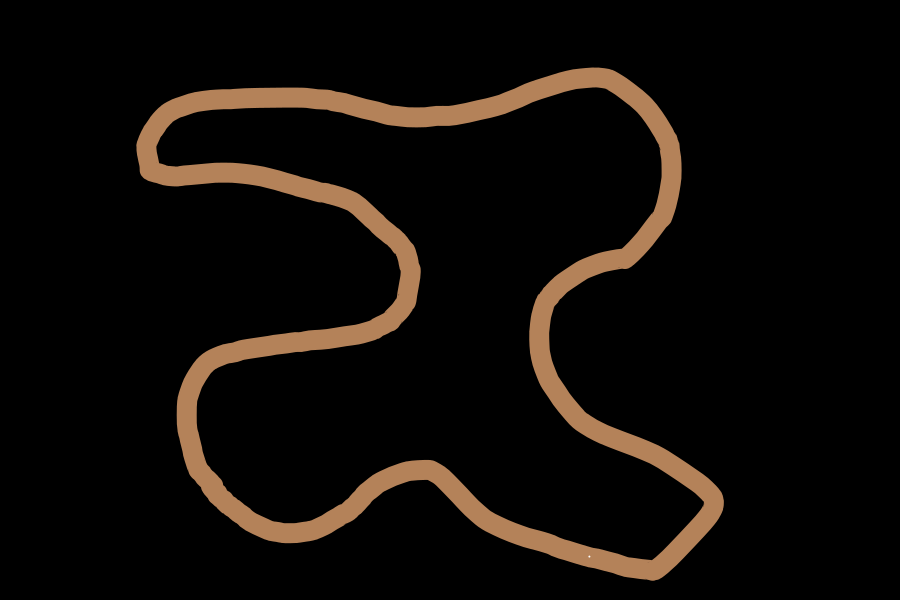
\includegraphics[width=5cm, height=4cm]{track_06.png}
		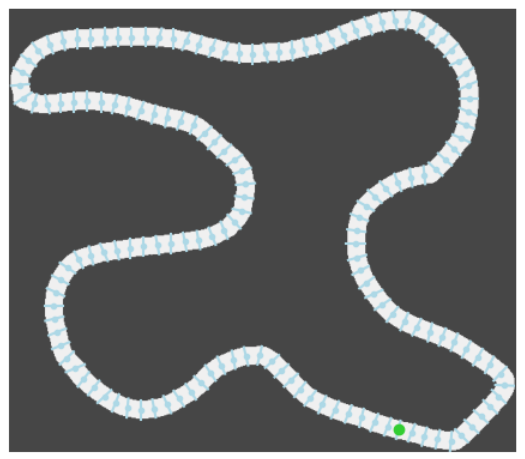
\includegraphics[width=5cm, height=4cm]{track_06_computed.png}
		\caption{\underline{.png and computed track}}
	\end{figure}
\end{center}

	
		\section{Cars' physics}
The Car physic is really simple. It is a 2D cartoon-like physics that act as follow:\\
The car has to main informations: its speed $\in [0,$ MaxSpeed$]$ and its rotation $\in [0,360]$. The physics is simple, at each times step, the car move to next coordinates on direction of the car's rotation and of a lenght equal to the car's speed.\\
If the coordinates of the car is $(x,y)$, its speed is $s$ and its rotation is $\alpha$, then, after a time step, the coordinate of the car will be:
\[(s.cos(\frac{\pi}{180}\alpha) + x,\; s.sin(\frac{\pi}{180}\alpha) + x)\]
\\
Moreover, at each time step, the car can make some actions:
\mlist{
\item it can accelerate, this will increase the car's speed by a constant
\item it can brake, this will decrease the car's speed by reduce the car speed by a constant. The car cannot have a negative speed.
\item it can turn, i.e. add a constant $\in \llbracket-K,K\rrbracket$ to its rotation. $K$ is a constant that is the maximum angle the car can turn per each time step.
}
The behaviour of the car will need to interact with the track therefore we need to decide what is the state of a car, i.e. how the car see the environment. We could give to our algorithms the track matrices, the informations of the car but this will leed to to many argument because a track can have size $900\times600$. Therefore we will need to train on all possible state wich will be at least $2^{900\times 600}$. Therefore, we decided to give a more realistic state wich represent how a car racer see. Then the state of a car is a array of size $8$.
\mlist{
\item $T_0$ is the current speed of the car
\item $\forall i\in\{1,...,7\}$, $T_i$ is the distance of the car to the next wall in the direction $\alpha + A_{i-1}$ where $\alpha$ is the current rotation of the car and $A=[60, 40, 20, 0, -20, -40, -60]$
}
Then, the representation looks like figure \ref{figure:car state}.
\begin{center}
\label{figure:car state}
	\begin{figure}[ht]
		\refstepcounter{fig}
		\centering
		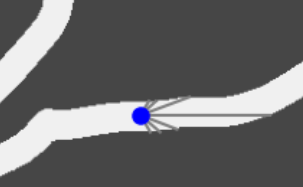
\includegraphics[width=4cm, height=3cm]{car_state.png}
		\caption{\underline{Car state}}
	\end{figure}
\end{center}
		
		\section{Technical aspects of the environment}
To manipulate our environment, we use the python packages \texttt{gymnasium} which provide code convention for those type or environment, i.e. environment where at each time step, you have one action to do. The environment has to have some essential function: \texttt{reset()} that reset the environment to be able to do an other simulation, \texttt{render()} that render the current state of our environment and the most important one is \texttt{step()} that do one step of time, i.e. given an action, the \texttt{step()} function figure out is the car has crashed or not, move the carn to its next position and return the new state of the car, a reward and if the car has crashed.\\
Our environment has a variable named \texttt{time} wich give us the opportunitie to discretise more or less the time.
		
		\section{Rewards}
For those type of problem where the AI model has to compute a behaviour, the AI model produces something which look like a function $f$ that take a car state and return an action. We need to specifie to our AI model when it produce a good action and a bad action, for instance, if a car crash, we need to punish the AI model.\\
We do that thanks to a function reward implemented in the function \texttt{step()} of our environment. The reward is an integer, the bigger it is the best the action was. To punished the car when it do something bad we do:
\mlist{
\item If the car crashes, we stop the simulation and return a reward of $-500$
\item If the car is not moving, i.e. has a speed of $0$, the reward is $-10$
}
For the positive reward, we have automatically computed some track line (represented in right image of figure \ref{figure:track}). If the car crosses next line, it has a reward of $+10\times$ the number of lines it has cross in the good order with this action. If the car cross a line in the wrong order, it means that it has gone backward, therefore, we punished the car with a reward of $-200$ and we stop the computation.\\
On top of that, at each time step, we add to the current reward the speed of the car divided by a constant to encourage the car to go fast.

		\section{Conclusion}
After explaining all of this, here is an example in figure \ref{figure:env example}. We have plot the trajectory of the car, the green color is when the car has accelerate, red color when it brake and yellow otherwise.
\begin{center}
\label{figure:env example}
	\begin{figure}[ht]
		\refstepcounter{fig}
		\centering
		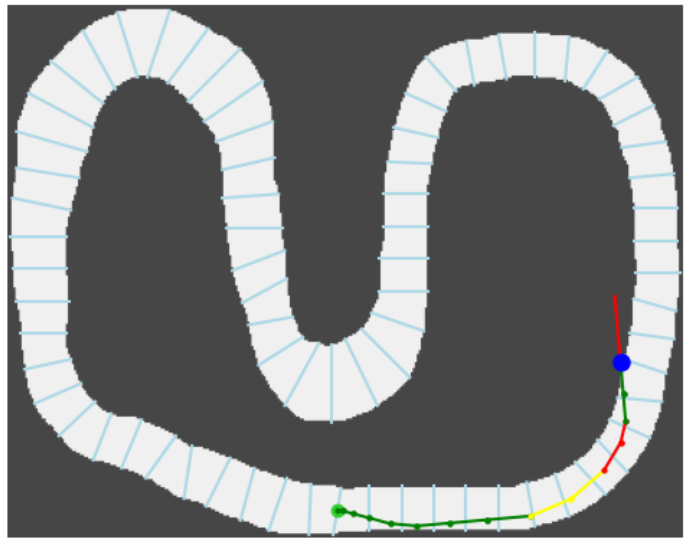
\includegraphics[width=6cm, height=5cm]{env_example.png}\\
		list of rounded reward: \texttt{[10, 1, 2, 12, 13, 13, 13, 14, 24, 14, 13, 12, 13, -497]}
		\caption{\underline{Car state}}
	\end{figure}
\end{center}
The total reward of a car behaviour is the sum of all reward of a simulation with a car behaviour.

	\part{Deep Q-learning}

		\section{Markovian decision process}
		We want to describe the interaction between an agent and its environment.
		In this report, a Markovian decision process is $(S,A,T,R)$ where :
		\begin{description}
			\item[$S$] is a set state in which our agent can be
			\item[$A$] is the set of actions our agent can take : all actions $a \in A$ are available from every state $s \in S$
			\item[$T$] is the transition function describing what is the next state of our agent after choosing one action : $T : S \times A \rightarrow S$
			\item[$R$] is the reward function giving   $R(s,a,s')$ if we go to $s'$ from $s$ by choosing action $a$
		\end{description}
 		
		\section{Q value}

		We can associate to a state a value that reflect the best cumulative reward that we can obtain 
		in the long run if a choose actions optimaly starting from its state. We call this value the Q-value of the state : $Q^*(s)$.

		\section{Deep Q-Learning}

		Deep Q-Learning is an algoirthm that aims at approximating $Q^*$ using a neural network.
							
		


	
	\part{Genetic algorithms}
		\section{What are genetic algorithms?}
Genetic algorithms (GA) are probabilistic algorithms based on natural selection. Therefore, GA takes some populations which are sets of solutions (here a solution is a car's behaviour), select the best solutions thanks to the reward function. Then, it changes the population by adding new random solutions, adding some mutations which are some small variations of a behaviour, adding some cross-over which are the equivalent of natural reproduction. We will repeat this process a fixed number of generations.
		
		\section{Markov Chain modelisation}
We will now introduce a Markov chain modelisation to genetic algorithm.\\
We define a markov chaine $(Y_n)_{n\in\mathbb{N}}$ as folowing:
\mlist{
\item A state of $(Y_n)_{n\in\mathbb{N}}$ is a population.
\item Let $y_0$ be a special state such that if $Y_n = y_0$ then it means that the population of state $Y_n$ contain an optimal solution.
}
Now, the sequence of population of genetic algorithm can be discribe with this markov chains. $Y_n$ represent the population at generation $n$.\\
Notice that the state $y_0$ is an absorbing state. In fact if $Y_n = y_0$ then it mean that $P_n[0]$ is optimal. Since we always kept the best solution of previous populations, it means that $\forall n'>n$, we have that $P_{n'}$ contain an optimal solution. Therefore, $\forall n'>n$, $Y_{n'} = y_0$. Moreover, $y_0$ is the only absorbing state of $(Y_n)_{n\in\mathbb{N}}$.\\
\\
If we suppose that our mutation and cross-over are made such that a solution $x$ can reach $y$ by a series of a finite number of those operations. Then, all solutions $x$ can reach an optimal value. Then every state $y_n$ can reach state $y_0$. The set of all possible state is finite.\\
Then $\mathbb{P}(Y_n = y_0) \underset{n \rightarrow +\infty}{\rightarrow} 1$\\
Then $\mathbb{P}($ The population $P_n$ contain an optimal solution$) \underset{n \rightarrow +\infty}{\rightarrow} 1$
		
		\section{NEAT}
Basic genetic algorithms are not efficient enought to compute an optimize behaviour. Therefore, we will use the famous python packages called \texttt{NEAT}. It is an optimized generalized genetic algorithms with dynamic neural network. By dynamic we mean that the algorithm can add or delete some of the nodes of the neural network. The principle of GA stay the same but we have a lot more hyperparameters.
	
	
	\part{Performance Evaluation}
	Once the models are selected (in this case, Deep Q-Learning and Genetic Algorithms), the next step is to compare them using various metrics. For this purpose, we choose the following metric: the average reward after training.

We measure this value across different training durations and varying numbers of tracks used for training the models. To ensure robustness and evaluate potential overfitting, we test the models on tracks that were not included in the training set. \\
This approach is applied in the context of an AI project where we train AI agents to complete a racing circuit. The goal is for the cars to complete laps as quickly as possible, and the average reward reflects their performance under these conditions.
		\section{GA VS Q}
		
		\section{Q hyperparameter}
		
		\section{Best car}



\end{document}